\section{Logical Network Segmentation}

The TAC Industries platform employs logical network segmentation using multiple VLANs to enforce separation of duties, reduce lateral movement, and align network reachability with trust boundaries. The design explicitly avoids flat network assumptions and enforces a deny-by-default posture between segments.

Enterprise-managed devices connect to the TAC-Inc Wi-Fi network, which is mapped to a restricted enterprise VLAN. Devices on this network are authenticated, monitored, and policy-controlled but are not granted direct access to core infrastructure services. Instead, access is limited to approved application endpoints and authentication services.

A separate guest wireless network (tguest) is provided for unmanaged or visitor devices. This network is fully isolated from internal systems and routed directly to the internet through perimeter controls. No east-west or internal access is permitted from the guest segment, ensuring that untrusted devices cannot interact with sensitive resources.

Additional VLANs are defined for core services, security tooling, bastion access, and administrative connectivity. Inter-VLAN routing is tightly controlled, and only explicitly permitted flows are allowed. This approach ensures that network segmentation supports Zero Trust principles by limiting blast radius and preventing implicit trust based on network location \cite{nist80053}.

\begin{figure}[!ht]
    \centering
    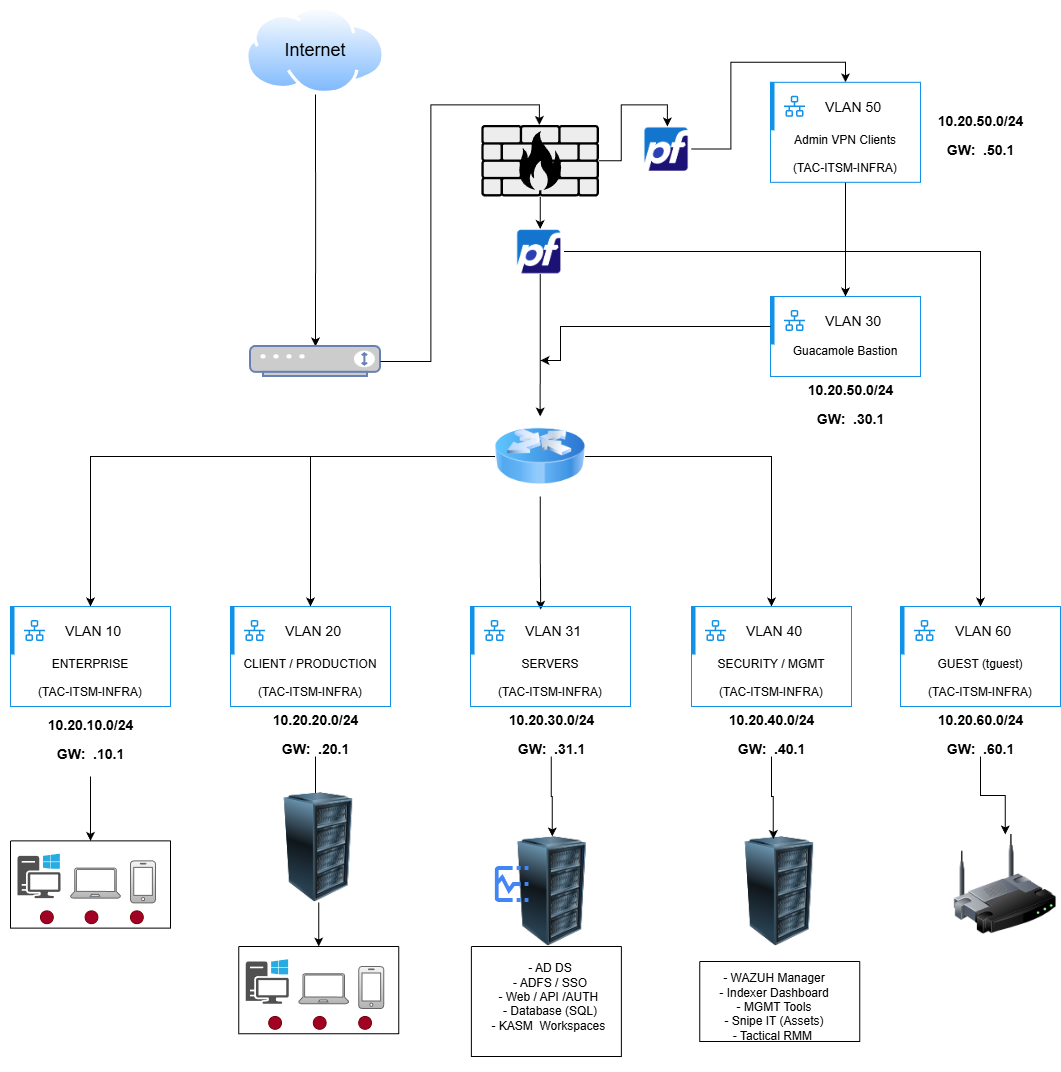
\includegraphics[width=\textwidth]{Images/1networkinfra.png}
    \caption{Logical VLAN Network segmentation and infrastructure overview}
    \label{fig:network-architecture}
\end{figure}


\section{Edge and Perimeter Security}

Perimeter security for TAC Industries is enforced using a dedicated firewall platform that acts as the central gateway between internal networks and external connectivity. The firewall provides stateful packet inspection, network address translation, and explicit traffic filtering between VLANs and the internet \cite{nist80094}.

All inbound access is denied by default, with only explicitly defined services exposed where required. Outbound traffic is similarly controlled to reduce data exfiltration risk and limit unnecessary external dependencies. Network address translation is used to prevent direct exposure of internal addressing schemes.

The pfSense firewall acts as the central enforcement point for network segmentation, VPN termination, firewalling, and selective proxying. All domain-enrolled enterprise devices route traffic through pfSense, enabling consistent policy enforcement and centralised logging. Firewall, proxy, and intrusion detection events are forwarded to the SIEM to support correlation and auditability\cite{pfsense}.

\vspace{1.5\baselineskip}


\begin{figure}[!ht]
    \centering
    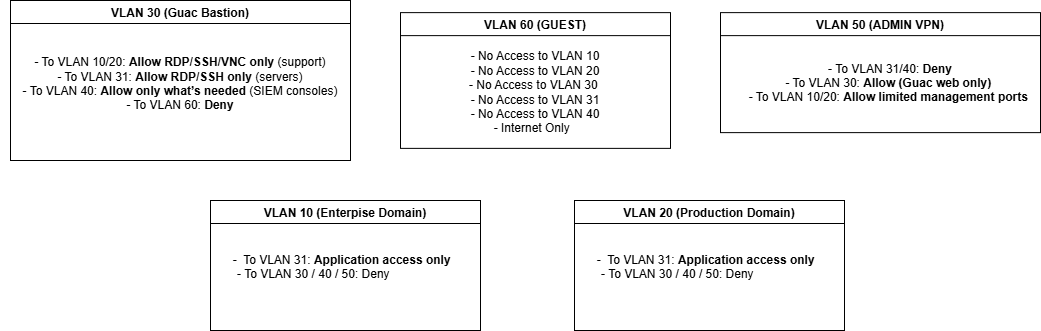
\includegraphics[width=\textwidth]{Images/VLAN-table.png}
    \caption{Logical VLAN Network segmentation and infrastructure overview}
    \label{fig:network-architecture}
\end{figure}

\section{Remote Access and Privileged Access Model}

Remote access to internal resources is brokered through a layered access model combining VPN authentication, bastion access, and application isolation. WireGuard, Windows IPSec VPN and OpenVPN servers provides encrypted traffic into a dedicated administrative VPN subnet, accessible only to authorized infrastructure roles.

Privileged administrative access is brokered through a dedicated bastion host environment using a remote access gateway. Administrators do not directly access servers or management interfaces from user networks or VPN endpoints. Instead, all interactive administrative sessions are initiated through the bastion server, enabling session control, logging, and auditability \cite{nist80053}.

For investigative and client-facing workflows, Kasm Workspaces provide isolated browser-based access to internal applications and external resources \cite{kasm}. These workspaces allow users to access the case management application and supporting tools without exposing internal services directly to endpoint devices. This approach reduces data leakage risk and ensures that access to sensitive systems occurs within a controlled execution environment.

\section{Virtualization and Hosting Overview}

The TAC Industries platform is hosted on a Proxmox Virtual Environment, providing a flexible and isolated virtualisation layer for all core services. Proxmox enables the separation of infrastructure components such as directory services, application servers, monitoring systems, and bastion hosts into discrete virtual machines, reducing the impact of compromise and supporting principle-of-least-privilege design \cite{proxmox}.

Virtualisation allows services with different trust and security requirements to be isolated at both the network and operating system level, while still operating on shared physical hardware. This approach reflects realistic small-enterprise deployments where budget constraints necessitate efficient resource utilisation without sacrificing security boundaries.

Proxmox was selected due to its open source licensing, support for enterprise-grade features such as role-based administration, snapshotting, and network segmentation, and its suitability for self-hosted environments. In the context of Semester One, Proxmox functions as an enabling platform that supports architectural validation rather than a focus of optimization or performance tuning.
